% Graphic for TeX using PGF
% Title: /home/guillaume/Documents/Université de Montréal/Automne 2014/Génie logiciel/Devoir/devoir-3/diagramme-de-classe-changement-1.dia
% Creator: Dia v0.97.3
% CreationDate: Sat Dec  6 11:14:53 2014
% For: guillaume
% \usepackage{tikz}
% The following commands are not supported in PSTricks at present
% We define them conditionally, so when they are implemented,
% this pgf file will use them.
\ifx\du\undefined
  \newlength{\du}
\fi
\setlength{\du}{15\unitlength}
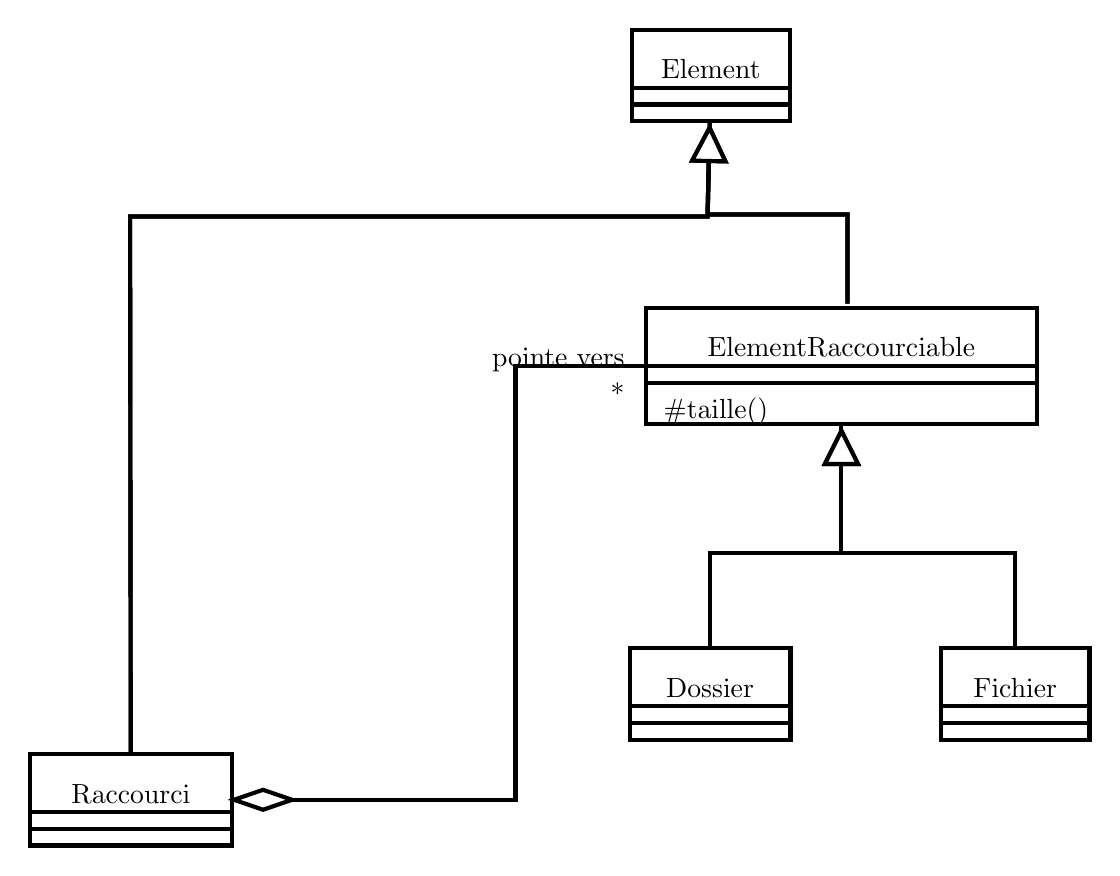
\begin{tikzpicture}
\pgftransformxscale{1.000000}
\pgftransformyscale{-1.000000}
\definecolor{dialinecolor}{rgb}{0.000000, 0.000000, 0.000000}
\pgfsetstrokecolor{dialinecolor}
\definecolor{dialinecolor}{rgb}{1.000000, 1.000000, 1.000000}
\pgfsetfillcolor{dialinecolor}
\pgfsetlinewidth{0.100000\du}
\pgfsetdash{}{0pt}
\definecolor{dialinecolor}{rgb}{1.000000, 1.000000, 1.000000}
\pgfsetfillcolor{dialinecolor}
\fill (31.100000\du,1.350000\du)--(31.100000\du,2.750000\du)--(34.912500\du,2.750000\du)--(34.912500\du,1.350000\du)--cycle;
\definecolor{dialinecolor}{rgb}{0.000000, 0.000000, 0.000000}
\pgfsetstrokecolor{dialinecolor}
\draw (31.100000\du,1.350000\du)--(31.100000\du,2.750000\du)--(34.912500\du,2.750000\du)--(34.912500\du,1.350000\du)--cycle;
% setfont left to latex
\definecolor{dialinecolor}{rgb}{0.000000, 0.000000, 0.000000}
\pgfsetstrokecolor{dialinecolor}
\node at (33.006250\du,2.300000\du){Element};
\definecolor{dialinecolor}{rgb}{1.000000, 1.000000, 1.000000}
\pgfsetfillcolor{dialinecolor}
\fill (31.100000\du,2.750000\du)--(31.100000\du,3.150000\du)--(34.912500\du,3.150000\du)--(34.912500\du,2.750000\du)--cycle;
\definecolor{dialinecolor}{rgb}{0.000000, 0.000000, 0.000000}
\pgfsetstrokecolor{dialinecolor}
\draw (31.100000\du,2.750000\du)--(31.100000\du,3.150000\du)--(34.912500\du,3.150000\du)--(34.912500\du,2.750000\du)--cycle;
\definecolor{dialinecolor}{rgb}{1.000000, 1.000000, 1.000000}
\pgfsetfillcolor{dialinecolor}
\fill (31.100000\du,3.150000\du)--(31.100000\du,3.550000\du)--(34.912500\du,3.550000\du)--(34.912500\du,3.150000\du)--cycle;
\definecolor{dialinecolor}{rgb}{0.000000, 0.000000, 0.000000}
\pgfsetstrokecolor{dialinecolor}
\draw (31.100000\du,3.150000\du)--(31.100000\du,3.550000\du)--(34.912500\du,3.550000\du)--(34.912500\du,3.150000\du)--cycle;
\pgfsetlinewidth{0.100000\du}
\pgfsetdash{}{0pt}
\definecolor{dialinecolor}{rgb}{1.000000, 1.000000, 1.000000}
\pgfsetfillcolor{dialinecolor}
\fill (16.600000\du,18.800000\du)--(16.600000\du,20.200000\du)--(21.470000\du,20.200000\du)--(21.470000\du,18.800000\du)--cycle;
\definecolor{dialinecolor}{rgb}{0.000000, 0.000000, 0.000000}
\pgfsetstrokecolor{dialinecolor}
\draw (16.600000\du,18.800000\du)--(16.600000\du,20.200000\du)--(21.470000\du,20.200000\du)--(21.470000\du,18.800000\du)--cycle;
% setfont left to latex
\definecolor{dialinecolor}{rgb}{0.000000, 0.000000, 0.000000}
\pgfsetstrokecolor{dialinecolor}
\node at (19.035000\du,19.750000\du){Raccourci};
\definecolor{dialinecolor}{rgb}{1.000000, 1.000000, 1.000000}
\pgfsetfillcolor{dialinecolor}
\fill (16.600000\du,20.200000\du)--(16.600000\du,20.600000\du)--(21.470000\du,20.600000\du)--(21.470000\du,20.200000\du)--cycle;
\definecolor{dialinecolor}{rgb}{0.000000, 0.000000, 0.000000}
\pgfsetstrokecolor{dialinecolor}
\draw (16.600000\du,20.200000\du)--(16.600000\du,20.600000\du)--(21.470000\du,20.600000\du)--(21.470000\du,20.200000\du)--cycle;
\definecolor{dialinecolor}{rgb}{1.000000, 1.000000, 1.000000}
\pgfsetfillcolor{dialinecolor}
\fill (16.600000\du,20.600000\du)--(16.600000\du,21.000000\du)--(21.470000\du,21.000000\du)--(21.470000\du,20.600000\du)--cycle;
\definecolor{dialinecolor}{rgb}{0.000000, 0.000000, 0.000000}
\pgfsetstrokecolor{dialinecolor}
\draw (16.600000\du,20.600000\du)--(16.600000\du,21.000000\du)--(21.470000\du,21.000000\du)--(21.470000\du,20.600000\du)--cycle;
\pgfsetlinewidth{0.100000\du}
\pgfsetdash{}{0pt}
\pgfsetmiterjoin
\pgfsetbuttcap
{
\definecolor{dialinecolor}{rgb}{0.000000, 0.000000, 0.000000}
\pgfsetfillcolor{dialinecolor}
% was here!!!
\definecolor{dialinecolor}{rgb}{0.000000, 0.000000, 0.000000}
\pgfsetstrokecolor{dialinecolor}
\draw (21.519766\du,19.900000\du)--(28.300000\du,19.900000\du)--(28.300000\du,9.450000\du)--(31.400932\du,9.450000\du);
}
\definecolor{dialinecolor}{rgb}{0.000000, 0.000000, 0.000000}
\pgfsetstrokecolor{dialinecolor}
\draw (22.778345\du,19.900000\du)--(28.300000\du,19.900000\du)--(28.300000\du,9.450000\du)--(31.400932\du,9.450000\du);
\pgfsetdash{}{0pt}
\pgfsetmiterjoin
\pgfsetbuttcap
\definecolor{dialinecolor}{rgb}{1.000000, 1.000000, 1.000000}
\pgfsetfillcolor{dialinecolor}
\fill (21.519766\du,19.900000\du)--(22.219766\du,19.660000\du)--(22.919766\du,19.900000\du)--(22.219766\du,20.140000\du)--cycle;
\pgfsetlinewidth{0.100000\du}
\pgfsetdash{}{0pt}
\pgfsetmiterjoin
\pgfsetbuttcap
\definecolor{dialinecolor}{rgb}{0.000000, 0.000000, 0.000000}
\pgfsetstrokecolor{dialinecolor}
\draw (21.519766\du,19.900000\du)--(22.219766\du,19.660000\du)--(22.919766\du,19.900000\du)--(22.219766\du,20.140000\du)--cycle;
% setfont left to latex
\definecolor{dialinecolor}{rgb}{0.000000, 0.000000, 0.000000}
\pgfsetstrokecolor{dialinecolor}
\node[anchor=west] at (28.400000\du,14.525000\du){};
\definecolor{dialinecolor}{rgb}{0.000000, 0.000000, 0.000000}
\pgfsetstrokecolor{dialinecolor}
\node[anchor=west] at (23.119766\du,19.750000\du){};
\definecolor{dialinecolor}{rgb}{0.000000, 0.000000, 0.000000}
\pgfsetstrokecolor{dialinecolor}
\node[anchor=east] at (31.200932\du,9.300000\du){ pointe vers};
\definecolor{dialinecolor}{rgb}{0.000000, 0.000000, 0.000000}
\pgfsetstrokecolor{dialinecolor}
\node[anchor=east] at (31.200932\du,10.100000\du){*};
\pgfsetlinewidth{0.100000\du}
\pgfsetdash{}{0pt}
\pgfsetmiterjoin
\pgfsetbuttcap
{
\definecolor{dialinecolor}{rgb}{0.000000, 0.000000, 0.000000}
\pgfsetfillcolor{dialinecolor}
% was here!!!
\definecolor{dialinecolor}{rgb}{0.000000, 0.000000, 0.000000}
\pgfsetstrokecolor{dialinecolor}
\draw (32.980244\du,3.599658\du)--(32.929341\du,5.850000\du)--(19.016789\du,5.850000\du)--(19.033509\du,18.750034\du);
}
\definecolor{dialinecolor}{rgb}{0.000000, 0.000000, 0.000000}
\pgfsetstrokecolor{dialinecolor}
\draw (32.959625\du,4.511228\du)--(32.929341\du,5.850000\du)--(19.016789\du,5.850000\du)--(19.033509\du,18.750034\du);
\pgfsetmiterjoin
\definecolor{dialinecolor}{rgb}{1.000000, 1.000000, 1.000000}
\pgfsetfillcolor{dialinecolor}
\fill (33.359522\du,4.520274\du)--(32.977716\du,3.711433\du)--(32.559727\du,4.502183\du)--cycle;
\pgfsetlinewidth{0.100000\du}
\pgfsetdash{}{0pt}
\pgfsetmiterjoin
\definecolor{dialinecolor}{rgb}{0.000000, 0.000000, 0.000000}
\pgfsetstrokecolor{dialinecolor}
\draw (33.359522\du,4.520274\du)--(32.977716\du,3.711433\du)--(32.559727\du,4.502183\du)--cycle;
% setfont left to latex
\pgfsetlinewidth{0.100000\du}
\pgfsetdash{}{0pt}
\definecolor{dialinecolor}{rgb}{1.000000, 1.000000, 1.000000}
\pgfsetfillcolor{dialinecolor}
\fill (31.450000\du,8.050000\du)--(31.450000\du,9.450000\du)--(40.855000\du,9.450000\du)--(40.855000\du,8.050000\du)--cycle;
\definecolor{dialinecolor}{rgb}{0.000000, 0.000000, 0.000000}
\pgfsetstrokecolor{dialinecolor}
\draw (31.450000\du,8.050000\du)--(31.450000\du,9.450000\du)--(40.855000\du,9.450000\du)--(40.855000\du,8.050000\du)--cycle;
% setfont left to latex
\definecolor{dialinecolor}{rgb}{0.000000, 0.000000, 0.000000}
\pgfsetstrokecolor{dialinecolor}
\node at (36.152500\du,9.000000\du){ElementRaccourciable};
\definecolor{dialinecolor}{rgb}{1.000000, 1.000000, 1.000000}
\pgfsetfillcolor{dialinecolor}
\fill (31.450000\du,9.450000\du)--(31.450000\du,9.850000\du)--(40.855000\du,9.850000\du)--(40.855000\du,9.450000\du)--cycle;
\definecolor{dialinecolor}{rgb}{0.000000, 0.000000, 0.000000}
\pgfsetstrokecolor{dialinecolor}
\draw (31.450000\du,9.450000\du)--(31.450000\du,9.850000\du)--(40.855000\du,9.850000\du)--(40.855000\du,9.450000\du)--cycle;
\definecolor{dialinecolor}{rgb}{1.000000, 1.000000, 1.000000}
\pgfsetfillcolor{dialinecolor}
\fill (31.450000\du,9.850000\du)--(31.450000\du,10.850000\du)--(40.855000\du,10.850000\du)--(40.855000\du,9.850000\du)--cycle;
\definecolor{dialinecolor}{rgb}{0.000000, 0.000000, 0.000000}
\pgfsetstrokecolor{dialinecolor}
\draw (31.450000\du,9.850000\du)--(31.450000\du,10.850000\du)--(40.855000\du,10.850000\du)--(40.855000\du,9.850000\du)--cycle;
% setfont left to latex
\definecolor{dialinecolor}{rgb}{0.000000, 0.000000, 0.000000}
\pgfsetstrokecolor{dialinecolor}
\node[anchor=west] at (31.600000\du,10.550000\du){\#taille()};
\pgfsetlinewidth{0.100000\du}
\pgfsetdash{}{0pt}
\definecolor{dialinecolor}{rgb}{1.000000, 1.000000, 1.000000}
\pgfsetfillcolor{dialinecolor}
\fill (38.550000\du,16.250000\du)--(38.550000\du,17.650000\du)--(42.130000\du,17.650000\du)--(42.130000\du,16.250000\du)--cycle;
\definecolor{dialinecolor}{rgb}{0.000000, 0.000000, 0.000000}
\pgfsetstrokecolor{dialinecolor}
\draw (38.550000\du,16.250000\du)--(38.550000\du,17.650000\du)--(42.130000\du,17.650000\du)--(42.130000\du,16.250000\du)--cycle;
% setfont left to latex
\definecolor{dialinecolor}{rgb}{0.000000, 0.000000, 0.000000}
\pgfsetstrokecolor{dialinecolor}
\node at (40.340000\du,17.200000\du){Fichier};
\definecolor{dialinecolor}{rgb}{1.000000, 1.000000, 1.000000}
\pgfsetfillcolor{dialinecolor}
\fill (38.550000\du,17.650000\du)--(38.550000\du,18.050000\du)--(42.130000\du,18.050000\du)--(42.130000\du,17.650000\du)--cycle;
\definecolor{dialinecolor}{rgb}{0.000000, 0.000000, 0.000000}
\pgfsetstrokecolor{dialinecolor}
\draw (38.550000\du,17.650000\du)--(38.550000\du,18.050000\du)--(42.130000\du,18.050000\du)--(42.130000\du,17.650000\du)--cycle;
\definecolor{dialinecolor}{rgb}{1.000000, 1.000000, 1.000000}
\pgfsetfillcolor{dialinecolor}
\fill (38.550000\du,18.050000\du)--(38.550000\du,18.450000\du)--(42.130000\du,18.450000\du)--(42.130000\du,18.050000\du)--cycle;
\definecolor{dialinecolor}{rgb}{0.000000, 0.000000, 0.000000}
\pgfsetstrokecolor{dialinecolor}
\draw (38.550000\du,18.050000\du)--(38.550000\du,18.450000\du)--(42.130000\du,18.450000\du)--(42.130000\du,18.050000\du)--cycle;
\pgfsetlinewidth{0.100000\du}
\pgfsetdash{}{0pt}
\definecolor{dialinecolor}{rgb}{1.000000, 1.000000, 1.000000}
\pgfsetfillcolor{dialinecolor}
\fill (31.050000\du,16.250000\du)--(31.050000\du,17.650000\du)--(34.927500\du,17.650000\du)--(34.927500\du,16.250000\du)--cycle;
\definecolor{dialinecolor}{rgb}{0.000000, 0.000000, 0.000000}
\pgfsetstrokecolor{dialinecolor}
\draw (31.050000\du,16.250000\du)--(31.050000\du,17.650000\du)--(34.927500\du,17.650000\du)--(34.927500\du,16.250000\du)--cycle;
% setfont left to latex
\definecolor{dialinecolor}{rgb}{0.000000, 0.000000, 0.000000}
\pgfsetstrokecolor{dialinecolor}
\node at (32.988750\du,17.200000\du){Dossier};
\definecolor{dialinecolor}{rgb}{1.000000, 1.000000, 1.000000}
\pgfsetfillcolor{dialinecolor}
\fill (31.050000\du,17.650000\du)--(31.050000\du,18.050000\du)--(34.927500\du,18.050000\du)--(34.927500\du,17.650000\du)--cycle;
\definecolor{dialinecolor}{rgb}{0.000000, 0.000000, 0.000000}
\pgfsetstrokecolor{dialinecolor}
\draw (31.050000\du,17.650000\du)--(31.050000\du,18.050000\du)--(34.927500\du,18.050000\du)--(34.927500\du,17.650000\du)--cycle;
\definecolor{dialinecolor}{rgb}{1.000000, 1.000000, 1.000000}
\pgfsetfillcolor{dialinecolor}
\fill (31.050000\du,18.050000\du)--(31.050000\du,18.450000\du)--(34.927500\du,18.450000\du)--(34.927500\du,18.050000\du)--cycle;
\definecolor{dialinecolor}{rgb}{0.000000, 0.000000, 0.000000}
\pgfsetstrokecolor{dialinecolor}
\draw (31.050000\du,18.050000\du)--(31.050000\du,18.450000\du)--(34.927500\du,18.450000\du)--(34.927500\du,18.050000\du)--cycle;
\pgfsetlinewidth{0.100000\du}
\pgfsetdash{}{0pt}
\pgfsetmiterjoin
\pgfsetbuttcap
{
\definecolor{dialinecolor}{rgb}{0.000000, 0.000000, 0.000000}
\pgfsetfillcolor{dialinecolor}
% was here!!!
\definecolor{dialinecolor}{rgb}{0.000000, 0.000000, 0.000000}
\pgfsetstrokecolor{dialinecolor}
\draw (36.152500\du,10.900354\du)--(36.152500\du,13.950037\du)--(32.988750\du,13.950037\du)--(32.988750\du,16.199719\du);
}
\definecolor{dialinecolor}{rgb}{0.000000, 0.000000, 0.000000}
\pgfsetstrokecolor{dialinecolor}
\draw (36.152500\du,11.812157\du)--(36.152500\du,13.950037\du)--(32.988750\du,13.950037\du)--(32.988750\du,16.199719\du);
\pgfsetmiterjoin
\definecolor{dialinecolor}{rgb}{1.000000, 1.000000, 1.000000}
\pgfsetfillcolor{dialinecolor}
\fill (36.552500\du,11.812157\du)--(36.152500\du,11.012157\du)--(35.752500\du,11.812157\du)--cycle;
\pgfsetlinewidth{0.100000\du}
\pgfsetdash{}{0pt}
\pgfsetmiterjoin
\definecolor{dialinecolor}{rgb}{0.000000, 0.000000, 0.000000}
\pgfsetstrokecolor{dialinecolor}
\draw (36.552500\du,11.812157\du)--(36.152500\du,11.012157\du)--(35.752500\du,11.812157\du)--cycle;
% setfont left to latex
\pgfsetlinewidth{0.100000\du}
\pgfsetdash{}{0pt}
\pgfsetmiterjoin
\pgfsetbuttcap
{
\definecolor{dialinecolor}{rgb}{0.000000, 0.000000, 0.000000}
\pgfsetfillcolor{dialinecolor}
% was here!!!
\definecolor{dialinecolor}{rgb}{0.000000, 0.000000, 0.000000}
\pgfsetstrokecolor{dialinecolor}
\draw (36.152500\du,10.900354\du)--(36.152500\du,13.950037\du)--(40.340000\du,13.950037\du)--(40.340000\du,16.199719\du);
}
\definecolor{dialinecolor}{rgb}{0.000000, 0.000000, 0.000000}
\pgfsetstrokecolor{dialinecolor}
\draw (36.152500\du,11.812157\du)--(36.152500\du,13.950037\du)--(40.340000\du,13.950037\du)--(40.340000\du,16.199719\du);
\pgfsetmiterjoin
\definecolor{dialinecolor}{rgb}{1.000000, 1.000000, 1.000000}
\pgfsetfillcolor{dialinecolor}
\fill (36.552500\du,11.812157\du)--(36.152500\du,11.012157\du)--(35.752500\du,11.812157\du)--cycle;
\pgfsetlinewidth{0.100000\du}
\pgfsetdash{}{0pt}
\pgfsetmiterjoin
\definecolor{dialinecolor}{rgb}{0.000000, 0.000000, 0.000000}
\pgfsetstrokecolor{dialinecolor}
\draw (36.552500\du,11.812157\du)--(36.152500\du,11.012157\du)--(35.752500\du,11.812157\du)--cycle;
% setfont left to latex
\pgfsetlinewidth{0.100000\du}
\pgfsetdash{}{0pt}
\pgfsetmiterjoin
\pgfsetbuttcap
{
\definecolor{dialinecolor}{rgb}{0.000000, 0.000000, 0.000000}
\pgfsetfillcolor{dialinecolor}
% was here!!!
\definecolor{dialinecolor}{rgb}{0.000000, 0.000000, 0.000000}
\pgfsetstrokecolor{dialinecolor}
\draw (32.979431\du,3.600336\du)--(32.928147\du,5.800000\du)--(36.300000\du,5.800000\du)--(36.300000\du,7.950000\du);
}
\definecolor{dialinecolor}{rgb}{0.000000, 0.000000, 0.000000}
\pgfsetstrokecolor{dialinecolor}
\draw (32.958179\du,4.511891\du)--(32.928147\du,5.800000\du)--(36.300000\du,5.800000\du)--(36.300000\du,7.950000\du);
\pgfsetmiterjoin
\definecolor{dialinecolor}{rgb}{1.000000, 1.000000, 1.000000}
\pgfsetfillcolor{dialinecolor}
\fill (33.358070\du,4.521215\du)--(32.976825\du,3.712109\du)--(32.558287\du,4.502568\du)--cycle;
\pgfsetlinewidth{0.100000\du}
\pgfsetdash{}{0pt}
\pgfsetmiterjoin
\definecolor{dialinecolor}{rgb}{0.000000, 0.000000, 0.000000}
\pgfsetstrokecolor{dialinecolor}
\draw (33.358070\du,4.521215\du)--(32.976825\du,3.712109\du)--(32.558287\du,4.502568\du)--cycle;
% setfont left to latex
\end{tikzpicture}
